%3
\section{Identification des activités et des tâches}
%Liste des ACTIVITES et des TACHES
%1 tâche = 1 étudiant et 1 semaine
%1 étudiant peut avoir plusieurs tâches la même semaine (en parallèle)
%PLAN DE CHARGES ( voir document spécifique )
%PLANNING ( DIAGRAMME DE GANTT )
%à l’aide d’un outil de gestion de projet : MS Project

\subsection{Schéma de déroulement général}

Selon le planning établi lors de la partie précédente, nous obtenons la liste des livrables.

\begin{center}
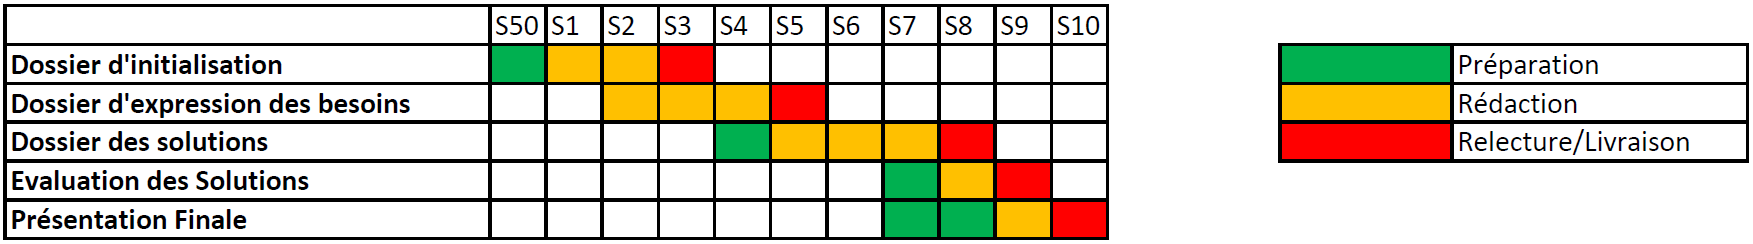
\includegraphics[width=17cm]{\PIXPATH/gantt}\hfill\\
\end{center}

\vfil
\pagebreak
\subsection{Liste des tâches par personne}

\subsubsection{Quentin Villers}

Les tâches d'encadrement comprennent des entrevues individuelles pour conduire l'équipe. 
Elles s'appliquent aussi bien au responsable qualité qu'aux membres de l'équipe. 

\begin{longtable}{|l|l|l|}
\hline
Semaine&Durée en H&Tâches\\
\endhead \hline
S00&1&Initialisation\\
\hline
S00&0,5&Réunion\\
\hline
S01&0,5&Réunion\\
\hline
S01&3&Pilotage\\
\hline
S01&3&Rédaction dossier d'initialisation\\
\hline
S02&0,5&Réunion\\
\hline
S02&2&Planification\\
\hline
S02&3&Encadrement\\
\hline
S03&0,5&Réunion\\
\hline
S03&2&Encadrement\\
\hline
S03&0,5&Recette PAQ\\
\hline
S03&1&Recette dossier d'initialisation\\
\hline
S03&0,5&Recette EDB -1\\
\hline
S04&0,5&Réunion\\
\hline
S04&2&Encadrement\\
\hline
S04&0,5&Recette \textsl{benchmarking}\\
\hline
S04&2&Synthèse du document\\
\hline
S05&0,5&Réunion\\
\hline
S05&2&Encadrement\\
\hline
S05&1&Recette dossier EDB complet\\
\hline
S05&1&Synthèse de S5\\
\hline
S06&0,5&Réunion\\
\hline
S06&1&Recette solution spécifique\\
\hline
S06&2&Encadrement\\
\hline
S07&0,5&Réunion\\
\hline
S07&1&Recette solution standard\\
\hline
S07&2&Encadrement\\
\hline
S07&2&Recette modélisation sur ARIS\\
\hline
S08&0,5&Réunion\\
\hline
S08&2&Encadrement\\
\hline
S08&4&Préparation du support de présentation final\\
\hline
S09&2&Répétition présentation\\
\hline
S09&1&Relecture du support de présentation\\
\hline
S09&6&Génération des bilans quantitatifs et qualitatifs\\
\hline
S10&4&Présentation finale\\
\hline
\end{longtable}

\pagebreak
\subsubsection{Raphaël Lizé}

Les tâches mentionnées comme de \textsl{soutien} vont permettre à Raphaël d'homogénéiser
la charge de l'équipe en fonction des difficultés rencontrées lors du travail. 
Ici sont mentionnées principalement les tâches inhérentes au rôle de responsable qualité,
l'adaptation de ces missions sera faite de manière agile.

\begin{longtable}{|l|l|l|}
\hline
Semaine&Durée en H&Tâches\\
\hline
S00&1&Initialisation\\
\hline
S00&0,5&Réunion\\
\hline
S01&0,5&Réunion\\
\hline
S01&3&Rédaction PAQ\\
\hline
S02&0,5&Réunion\\
\hline
S02&1&Gestion GIT\\
\hline
S02&5&Rédaction PAQ\\
\hline
S03&0,5&Réunion\\
\hline
S03&1&Recette PAQ\\
\hline
S03&2&Soutien\\
\hline
S03&1&Recette dossier d'initialisation\\
\hline
S04&0,5&Réunion\\
\hline
S04&2&Soutien\\
\hline
S04&1&Intégration des comptes rendus S2 et S3\\
\hline
S05&0,5&Réunion\\
\hline
S05&1&Aide à la réalisation\\
\hline
S05&2&Spécification de la solution spécifique\\
\hline
S05&1&Recette Dossier EDB complet\\
\hline
S05&0,5&Création modèle document solution spécifique\\
\hline
S06&0,5&Réunion\\
\hline
S06&1&Recette solution spécifique\\
\hline
S06&2&Modélisation ARIS\\
\hline
S06&0,5&Création modèle document solution standard\\
\hline
S07&0,5&Réunion\\
\hline
S07&1&Recette solution standard\\
\hline
S07&2&Modélisation\\
\hline
S07&2&Analyse cohérence des résultats\\
\hline
S08&3&Soutien\\
\hline
S08&0,5&Réunion\\
\hline
S08&0,5&Création modèle document choix de solution\\
\hline
S09&2&Répétition présentation\\
\hline
S09&1&Relecture support de présentation\\
\hline
S09&4&Aider Quentin\\
\hline
S10&4&Présentation finale\\
\hline
\end{longtable}

\pagebreak
\subsubsection{Karen Abanto}

Les temps affectés à Karen sont jugés comme plus long. Karen aura plus de travail
personnel pour arriver au niveau de résultat attendu. 
Le chef de projet l'encadrera de façon active.

\begin{longtable}{|l|l|l|}
\hline
Semaine&Durée en H&Tâches\\
\hline
S00&1&Initialisation\\
\hline
S00&0,5&Réunion\\
\hline
S01&0,5&Réunion\\
\hline
S01&3&Rédaction dossier d'initialisation\\
\hline
S02&0,5&Réunion\\
\hline
S02&5&Rédaction EDB - 1 Matériau\\
\hline
S02&2&Conclusion S2\\
\hline
S03&0,5&Réunion\\
\hline
S03&0,5&Formation \textsl{benchmarking}\\
\hline
S03&4&\textsl{Benchmarking}\\
\hline
S04&0,5&Réunion\\
\hline
S04&4&Analyse des dysfonctionnements\\
\hline
S05&0,5&Réunion\\
\hline
S05&4&Spécification de la solution spécifique\\
\hline
S06&0,5&Réunion\\
\hline
S06&4&Configuration SAP\\
\hline
S07&0,5&Réunion\\
\hline
S07&4&Modélisation sur ARIS\\
\hline
S08&0,5&Réunion\\
\hline
S08&4&Choix du projet plus organisation de la suite\\
\hline
S09&2&Répétition présentation\\
\hline
S10&4&Présentation finale\\
\hline
\end{longtable}


\pagebreak
\subsubsection{Clément Geiger}
\begin{longtable}{|l|l|l|}
\endhead \hline
Semaine&Durée en H&Tâches\\
\hline
S00&1&Initialisation\\
\hline
S00&0,5&Réunion\\
\hline
S01&0,5&Réunion\\
\hline
S01&3&Rédaction dossier d'initialisation\\
\hline
S02&0,5&Réunion\\
\hline
S02&1&Gestion GIT\\
\hline
S02&2&Rédaction EDB - 1 Achat\\
\hline
S02&1&Conclusion S2\\
\hline
S03&0,5&Réunion\\
\hline
S03&0,5&Formation \textsl{benchmarking}\\
\hline
S03&2&\textsl{Benchmarking}\\
\hline
S04&0,5&Réunion\\
\hline
S04&3&Règles de gestion principales\\
\hline
S05&0,5&Réunion\\
\hline
S05&1&Spécification de la solution spécifique\\
\hline
S05&2&Modélisation\\
\hline
S06&0,5&Réunion\\
\hline
S06&3&Modélisation sur ARIS\\
\hline
S07&0,5&Réunion\\
\hline
S07&3&Modélisation sur ARIS\\
\hline
S08&0,5&Réunion\\
\hline
S08&3&Calculs des gains et ROI\\
\hline
S08&2&Comparaison des solutions\\
\hline
S09&2&Répétition présentation\\
\hline
S10&4&Présentation finale\\
\hline
\end{longtable}

\pagebreak
\subsubsection{Hugo Pastore de Cristofaro}

\begin{longtable}{|l|l|l|}
\endhead \hline
Semaine&Durée en H&Tâches\\
\hline
S00&1&Initialisation\\
\hline
S00&0,5&Réunion\\
\hline
S01&0,5&Réunion\\
\hline
S01&2&Rédaction PAQ\\
\hline
S01&1&Rédaction dossier d'initialisation\\
\hline
S02&0,5&Réunion\\
\hline
S02&1&\textsl{Benchmarking}\\
\hline
S02&2&Maintenance\\
\hline
S02&1&Rédaction PAQ\\
\hline
S03&0,5&Réunion\\
\hline
S03&0,5&Formation \textsl{benchmarking}\\
\hline
S03&2&\textsl{Benchmarking}\\
\hline
S03&2&Conclusion S3 \textsl{benchmarking}\\
\hline
S04&0,5&Réunion\\
\hline
S04&3&Modèle de données\\
\hline
S05&0,5&Réunion\\
\hline
S05&1&Spécification de la solution spécifique\\
\hline
S05&2&Modélisation\\
\hline
S06&0,5&Réunion\\
\hline
S06&4&Configuration SAP\\
\hline
S07&0,5&Réunion\\
\hline
S07&4&Modélisation sur ARIS\\
\hline
S08&0,5&Réunion\\
\hline
S08&1&Chiffrage solution standard\\
\hline
S08&5&Préparation du support de présentation final\\
\hline
S09&2&Répétition présentation\\
\hline
S09&1&Relecture support de présentation\\
\hline
S10&4&Présentation finale\\
\hline
\end{longtable}

\pagebreak

